\documentclass[a4paper,12pt]{article}
\usepackage[utf8]{inputenc}
\usepackage{amsmath}
\usepackage{graphicx}
\usepackage{listings}
\usepackage{caption}
\usepackage{float}
\usepackage{tikz}
\usepackage{pgfplots}
\pgfplotsset{compat=1.18}
\usepackage{longtable}
\usepackage{pgfplots}
\usepackage{xcolor}
\lstdefinestyle{mystyle}{
    keywordstyle=\color{blue},       % kolor słów kluczowych
    numberstyle=\tiny\color{gray},   % kolor numerów linii
    basicstyle=\ttfamily\footnotesize, % styl podstawowy
    breaklines=true,                 % łamanie długich wierszy
    captionpos=b,                    % pozycja podpisu
    numbers=left,                    % numery linii po lewej stronie
    numbersep=1pt,                   % odstęp numerów linii
    showspaces=false,                % nie pokazuj spacji
    tabsize=2                        % rozmiar tabulacji
}

\lstset{style=mystyle}

\title{Analiza Algorytmów Sortowania}
\author{Ksawery Józefowski\\Politechnika Wrocławska}
\date{\today}

\begin{document}

\maketitle

\tableofcontents
\newpage

\section{Wstęp}
W ramach Listy 1 zaimplementowano i przeanalizowano trzy klasyczne algorytmy sortowania: \textit{Insertion Sort}, \textit{Merge Sort} oraz \textit{Heap Sort}. Każdy z algorytmów został zmodyfikowany: \textit{Insertion Sort} wstawia jednocześnie dwa elementy, \textit{Merge Sort} dzieli dane na trzy części zamiast dwóch, a \textit{Heap Sort} korzysta z kopców ternarnych. Celem projektu jest analiza wydajności algorytmów pod względem liczby porównań i przypisań dla różnych rozmiarów danych.

\section{Fragmenty Kodów}
Poniżej przedstawiono najciekawsze fragmenty kodu dla wybranych algorytmów.

\subsection{Insertion Sort z Wstawianiem Dwóch Elementów}
Klasyczny algorytm \textit{Insertion Sort} działa poprzez iteracyjne wstawianie kolejnych elementów do uporządkowanej części tablicy, przesuwając większe elementy, aby zrobić miejsce na nowy element. Modyfikacja wprowadzona w tym algorytmie polega na jednoczesnym wstawianiu dwóch kolejnych elementów:
\begin{itemize}
    \item Dwa kolejne elementy z nieuporządkowanej części są najpierw porównywane, aby ustalić ich kolejność.
    \item Następnie większy z nich jest wstawiany na pozycję bardziej wysuniętą w kierunku końca tablicy.
    \item Proces wstawiania odbywa się iteracyjnie, gdzie każdy z dwóch elementów porównywany jest z kolejnymi elementami uporządkowanej części tablicy i wstawiany na odpowiednie miejsce.
\end{itemize}

Dzięki temu podejściu liczba operacji wstawiania może zostać zmniejszona, gdyż jednocześnie przetwarzane są dwa elementy.

\newpage
\begin{lstlisting}[language=C++,caption=Insertion Sort z wstawianiem dwóch elementów]
void insertionSortDouble(float arr[], int n, int& comparisons, int& assignments) {    
    for (int i = 2; i < n; i += 2) {
        float key1 = arr[i];
        float key2 = arr[i - 1];
        assignments += 2;

        if (++comparisons && key1 < key2) {
            std::swap(key1, key2);
            assignments += 3;
        }

        int j = i - 2;

        while (j >= 0 && ++comparisons && arr[j] > key1) {
            arr[j + 2] = arr[j];
            assignments++;
            j--;
        }

        arr[j + 2] = key1;
        assignments++;
        
        while (j >= 0 && ++comparisons && arr[j] > key2) {
            arr[j + 1] = arr[j];
            assignments++;
            j--;
        }

        arr[j + 1] = key2;
        assignments++;
    }
    if (n % 2 == 0) {
        int lastKey = arr[n - 1];
        assignments++;
        int j = n - 2;

        while (j >= 0 && ++comparisons && arr[j] > lastKey) {
            arr[j + 1] = arr[j];
            assignments++;
            j--;
        }
        
        arr[j + 1] = lastKey;
        assignments++;
    }
}

\end{lstlisting}

\subsection{Merge Sort z Podziałem na Trzy Części}
Algorytm \textit{Merge Sort} w klasycznej wersji dzieli tablicę na dwie części, które są rekurencyjnie sortowane, a następnie łączone w uporządkowany sposób. Modyfikacja polega na dzieleniu tablicy na trzy części, co zmienia strukturę rekurencyjnych wywołań:
\begin{itemize}
    \item Tablica jest dzielona na trzy części o zbliżonej liczbie elementów.
    \item Każda z części jest sortowana rekurencyjnie za pomocą \textit{Merge Sort}.
    \item Po zakończeniu sortowania każda z trzech części jest łączona w jedną, uporządkowaną całość.
\end{itemize}

Zmiana ta powoduje, że podczas łączenia musimy operować na trzech posortowanych fragmentach, co zwiększa złożoność procesu scalania, ponieważ liczba operacji porównawczych wzrasta. Z drugiej strony zmniejsza się liczba poziomów rekurencji, co może przyspieszyć algorytm.
\newpage
\begin{lstlisting}[language=C++,caption=Merge Sort z podziałem na trzy części]
void mergeSort3way(float arr[], int left, int right, int& comparisons, int& assignments) {
    if (left < right) {
        comparisons++;
        int third = (right - left) / 3;
        int mid1 = left + third;
        int mid2 = right - third;

        mergeSort3way(arr, left, mid1, comparisons, assignments);
        mergeSort3way(arr, mid1 + 1, mid2, comparisons, assignments);
        mergeSort3way(arr, mid2 + 1, right, comparisons, assignments);

        merge3way(arr, left, mid1, mid2, right, comparisons, assignments);
    }
}
\end{lstlisting}

\subsection{Heap Sort z Kopcem Ternarnym}
Algorytm \textit{Heap Sort} opiera się na koncepcji kopca binarnego – struktury danych, w której każdy węzeł ma co najwyżej dwóch potomków, a klucz rodzica jest większy lub równy kluczom jego potomków (kopiec maksymalny). Klasyczny \textit{Heap Sort} składa się z dwóch głównych etapów:
\begin{itemize}
    \item \textbf{Budowanie kopca}: Tablica wejściowa jest przekształcana w kopiec maksymalny.
    \item \textbf{Sortowanie}: Największy element (szczyt kopca) jest zamieniany z ostatnim elementem tablicy, a kopiec jest ponownie porządkowany, aby zachować właściwość kopca.
\end{itemize}

W modyfikacji \textit{Heap Sort} zastosowano kopiec ternarny, w którym każdy węzeł może mieć do trzech potomków. Dzięki tej zmianie zmniejsza się głębokość kopca, co wpływa na zmniejszenie liczby operacji porównawczych przy wyprowadzaniu największego elementu na szczyt kopca. 

\newpage
Poniżej przedstawiono fragment kodu implementującego \textit{Heap Sort} z kopcem ternarnym:

\begin{lstlisting}[language=C++,caption=Heap Sort z kopcem ternarnym]
void ternaryHeapify(float arr[], int n, int i, int& comparisons, int& assignments) {
    int largest = i;
    int left = 3 * i + 1;
    int middle = 3 * i + 2;
    int right = 3 * i + 3;

    if (left < n && ++comparisons && arr[left] > arr[largest]) largest = left;
    if (middle < n && ++comparisons && arr[middle] > arr[largest]) largest = middle;
    if (right < n && ++comparisons && arr[right] > arr[largest]) largest = right;

    if (largest != i) {
        std::swap(arr[i], arr[largest]);
        assignments += 3;
        ternaryHeapify(arr, n, largest, comparisons, assignments);
    }
}

void ternaryHeapSort(float arr[], int n, int& comparisons, int& assignments) {
    for (int i = n / 3; i >= 0; --i) ternaryHeapify(arr, n, i, comparisons, assignments);

    for (int i = n - 1; i >= 0; --i) {
        std::swap(arr[0], arr[i]);
        assignments += 3;
        ternaryHeapify(arr, i, 0, comparisons, assignments);
    }
}
\end{lstlisting}
\newpage
\section{Analiza i Wyniki}
Testy przeprowadzono na losowych tablicach o rozmiarach 1000, 5000, 10000 elementów. Dla każdego algorytmu zliczono liczbę porównań oraz przypisań.

\subsection{Tabela Wyników}
\begin{longtable}{|c|c|c|c|c|}
\hline
Rozmiar danych & Algorytm & Porównania & Przypisania \\
\hline
10 & Insertion Sort & 18 & 27 \\
10 & Insertion Sort (Double) & 16 & 27 \\
10 & Merge Sort & 22 & 68 \\
10 & Merge Sort (Three-Way) & 37 & 55 \\
10 & Heap Sort & 37 & 78 \\
10 & Heap Sort (Ternary) & 41 & 46 \\
\hline
10000 & Insertion Sort & 24886600 & 24896608 \\
10000 & Insertion Sort (Double) & 12312894 & 12327768 \\
10000 & Merge Sort & 120429 & 267232 \\
10000 & Merge Sort (Three-Way) & 226002 & 166360 \\
10000 & Heap Sort & 235363 & 372447 \\
10000 & Heap Sort (Ternary) & 226431 & 166800 \\
\hline
100000 & Insertion Sort & 1450825191 & 1450946597 \\
100000 & Insertion Sort (Double) & 1250835994 & 1250985962 \\
100000 & Merge Sort & 1536358 & 3337856 \\
100000 & Merge Sort (Three-Way) & 2886413 & 2094331 \\
100000 & Heap Sort & 3019604 & 4724586 \\
100000 & Heap Sort (Ternary) & 2897214 & 2090924 \\
\hline
\caption{Porównanie liczby operacji dla różnych rozmiarów danych}
\label{tab:results}
\end{longtable}

\subsection{Wykresy Wyników}
Poniżej przedstawiono wykresy liczby porównań i przypisań dla poszczególnych algorytmów w zależności od rozmiaru danych.

\begin{figure}[H]
    \centering
    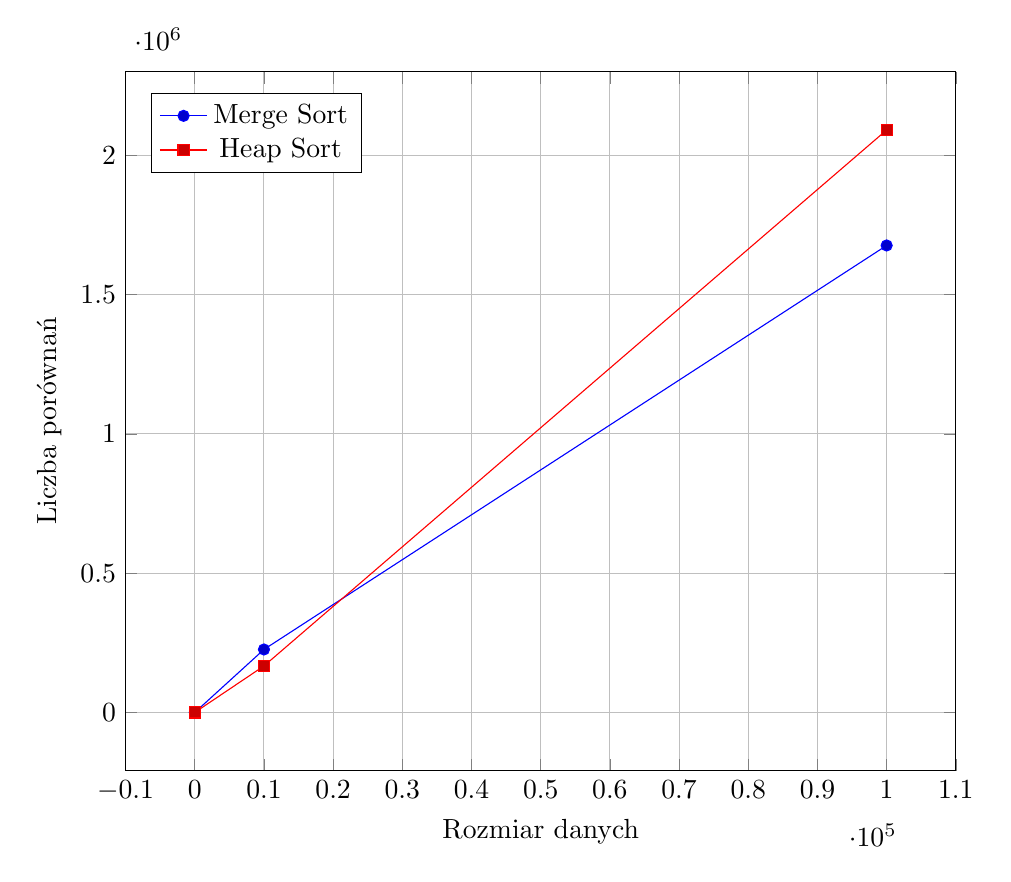
\begin{tikzpicture}
        \begin{axis}[
            width=\textwidth,
            xlabel={Rozmiar danych},
            ylabel={Liczba porównań},
            legend pos=north west,
            grid=major,
        ]
        
        \addplot coordinates {(10, 55 ) (10000, 226002 ) (100000, 1676330 )};
        \addplot coordinates {(10, 46 ) (10000, 166800 ) (100000, 2090924 )};
        \legend{Merge Sort, Heap Sort}
        \end{axis}
    \end{tikzpicture}
    \caption{Liczba porównań w zależności od rozmiaru danych}
\end{figure}

\begin{figure}[H]
    \centering
    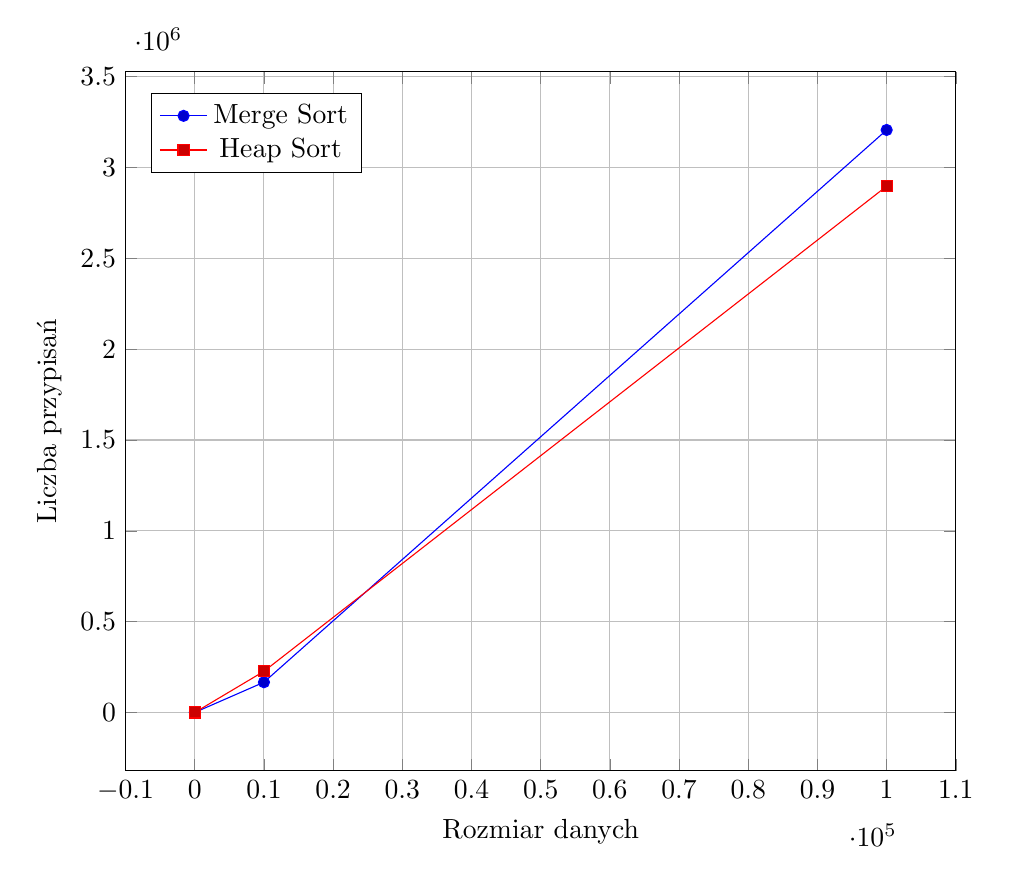
\begin{tikzpicture}
        \begin{axis}[
            width=\textwidth,
            xlabel={Rozmiar danych},
            ylabel={Liczba przypisań},
            legend pos=north west,
            grid=major,
        ]
        
        \addplot coordinates {(10, 37 ) (10000, 166360 ) (100000, 3206783 )};
        \addplot coordinates {(10, 41 ) (10000, 226431 ) (100000, 2897214 )};
        \legend{Merge Sort, Heap Sort}
        \end{axis}
    \end{tikzpicture}
    \caption{Liczba przypisań w zależności od rozmiaru danych}
\end{figure}

\section{Wnioski}
Przeprowadzona analiza wykazała, że:
\begin{itemize}
    \item \textit{Insertion Sort} z wstawianiem dwóch elementów zmniejsza liczbę operacji dla małych zestawów danych, lecz staje się mniej efektywny przy dużych rozmiarach tablicy.
    \item \textit{Merge Sort} z podziałem na trzy części zwiększa złożoność algorytmu, co skutkuje większą liczbą porównań, ale zmniejsza liczbę przypisań w porównaniu do tradycyjnego \textit{Merge Sort}.
    \item \textit{Heap Sort} z kopcem ternarnym zmniejsza głębokość kopca, co skraca liczbę operacji porównawczych przy dużych zbiorach danych, jednak zwiększa liczbę przypisań.
\end{itemize}

Z tego względu, klasyczna wersja \textit{Merge Sort} okazała się najbardziej efektywna przy dużych danych, zachowując korzystną równowagę między liczbą porównań a liczbą przypisań.

\end{document}
